\section{Optimierung der Empfehlungsqualität}
% V-Ansatz Teil 3 – Evaluation und Optimierung

\subsection{Zielfunktion und Evaluationsmetriken}
% Precision@5
% APS (Articles per Session)
% Begrenzte Zusatzmetriken (Diversity, Serendipity)

\subsection{Modellvarianten}
% CBF-Modell
% CF-Modell (z. B. LightFM, ALS)
% Hybridmodell (Score-Fusion: $\alpha \cdot \text{CBF} + (1 - \alpha) \cdot \text{CF}$)

\subsection{Optimierungsstrategie}
% α-Tuning (Score Fusion)
% Vergleichsbaselines
% Evaluation mit GA4-Daten

\subsection{Ergebnisse}
% Tabellen: Precision@5, APS je α
% Inhalt von: content/tables/vergleich_baselines.tex

\begin{table}[htbp]
    \centering
    \caption{Vergleich des optimierten Hybrid-Modells mit den Baseline-Modellen anhand der Metriken NDCG@10 und Hit Rate@10.}
    \label{tab:baseline_vergleich}
    \begin{tabular}{lrr}
        \toprule
        \textbf{Modell} & \textbf{NDCG@10} & \textbf{Hit Rate@10} \\
        \midrule
        Hybrid-Modell & 1.25\% & 1.8\% \\
        Popularity-Baseline        & 0.23\% & 0.6\% \\
        Recency-Baseline           & 0.14\% & 0.4\% \\
        \bottomrule
    \end{tabular}
\end{table}
% Visualisierungen: Liniendiagramme, ggf. UMAP-Spaces

\subsection{Interpretation und Analyse}
% Hybridisierung wirkungsvoll?
% Trade-offs und Nutzenklärung
% Ablationsidee: z. B. Ausschalten von CBF-/CF-Signal
% content/figures/plot_2d_performance.tex

\begin{figure}[htbp]
    \centering
    \includegraphics[width=0.9\textwidth]{content/figures/svg/2d_performance.pdf}
    \caption{2D-Darstellung des Hyperparameterraums. Die Achsen zeigen die Gewichtungen für das CBF- (\(w_{cbf}\)) und CF-Modell (\(w_{cf}\)). Die Farbe der Punkte indiziert den erreichten NDCG@10-Score. Der optimale Punkt ist markiert.}
    \label{fig:2d_performance}
\end{figure}
% content/figures/plot_3d_scatter.tex

\begin{figure}[htbp]
    \centering
    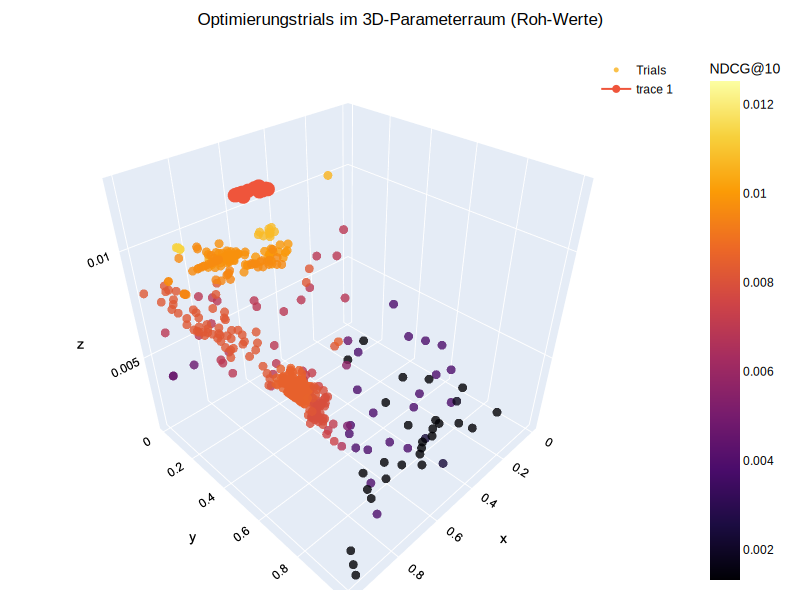
\includegraphics[width=0.8\textwidth]{content/figures/svg/3d_scatter_plot.pdf}
    \caption{Interaktives 3D-Streudiagramm der Optuna-Trials zur Visualisierung der Parameterabhängigkeiten. (Hinweis: Die Darstellung in der PDF-Version der Arbeit ist eine statische Ansicht).}
    \label{fig:3d_scatter}
\end{figure}
% content/figures/plot_kontour.tex

\begin{figure}[H]
    \centering
    \includegraphics[width=0.9\textwidth]{content/figures/svg/kontourplot.pdf}
    \caption{Konturplot zur Darstellung der NDCG@10-Verteilung im zweidimensionalen Parameterraum der Modellgewichtungen. Die Isolinien verbinden Bereiche mit ähnlicher Performance.}
    \label{fig:kontourplot}
\end{figure}
% content/figures/plot_optimierungsverlauf.tex

\begin{figure}[htbp]
    \centering
    \includegraphics[width=0.9\textwidth]{content/figures/svg/optimierungsverlauf.pdf}
    \caption{Visualisierung des Optimierungsverlaufs der 515 Optuna-Trials. Jeder Punkt stellt die NDCG@10-Metrik (Y-Achse) für einen bestimmten Trial (X-Achse) dar. Der Verlauf zeigt die Konvergenz des Optimierers gegen bessere Werte.}
    \label{fig:optimierungsverlauf}
\end{figure}
% content/figures/plot_hyperparameterraum.tex

\begin{figure}[H]
    \centering
    \includegraphics[width=0.9\textwidth]{content/figures/svg/hyperparameterraum.pdf}
    \caption{Visualisierung des zweidimensionalen Hyperparameterraums der Modellgewichtungen. Die Achsen repräsentieren die Gewichte für das CBF-Modell (\(w_{cbf}\)) und das CF-Modell (\(w_{cf}\)). Die Einfärbung der Punkte visualisiert den resultierenden NDCG@10-Wert für jede Konfiguration aus dem Optuna-Suchlauf.}
    \label{fig:hyperparameterraum}
\end{figure}